% This example is meant to be compiled with lualatex or xelatex
% The theme itself also supports pdflatex
\PassOptionsToPackage{unicode}{hyperref}
\documentclass[aspectratio=1610, 12pt]{beamer}

% Warning, if another latex run is needed
% \usepackage[aux]{rerunfilecheck}

% just list chapters and sections in the toc, not subsections or smaller
\setcounter{tocdepth}{1}

%------------------------------------------------------------------------------
%------------------------------ Fonts, Unicode, Language ----------------------
%------------------------------------------------------------------------------
\usepackage{fontspec}
\defaultfontfeatures{Ligatures=TeX}  % -- becomes en-dash etc.

% german language
\usepackage{polyglossia}
\setdefaultlanguage{german}

% for english abstract and english titles in the toc
\setotherlanguages{english}

% intelligent quotation marks, language and nesting sensitive
\usepackage[autostyle]{csquotes}

% microtypographical features, makes the text look nicer on the small scale
\usepackage{microtype}

%------------------------------------------------------------------------------
%------------------------ Math Packages and settings --------------------------
%------------------------------------------------------------------------------

\usepackage{amsmath}
\usepackage{amssymb}
\usepackage{mathtools}
\usepackage{bbold}

% Enable Unicode-Math and follow the ISO-Standards for typesetting math
\usepackage[
  math-style=ISO,
  bold-style=ISO,
  sans-style=italic,
  nabla=upright,
  partial=upright,
]{unicode-math}
\setmathfont{Latin Modern Math}

% nice, small fracs for the text with \sfrac{}{}
\usepackage{xfrac}


%------------------------------------------------------------------------------
%---------------------------- Numbers and Units -------------------------------
%------------------------------------------------------------------------------

\usepackage[
  locale=DE,
  separate-uncertainty=true,
  per-mode=symbol-or-fraction,
]{siunitx}
\sisetup{math-micro=\text{µ},text-micro=µ}
% \sisetup{tophrase={{ to }}}
%------------------------------------------------------------------------------
%-------------------------------- tables  -------------------------------------
%------------------------------------------------------------------------------

\usepackage{booktabs}       % \toprule, \midrule, \bottomrule, etc

%------------------------------------------------------------------------------
%-------------------------------- graphics -------------------------------------
%------------------------------------------------------------------------------

\usepackage{graphicx}
%\usepackage{rotating}
\usepackage{grffile}
\usepackage{tikz}
\usepackage{circuitikz}
\usepackage{tikz-feynman}
\usepackage{subcaption}

% allow figures to be placed in the running text by default:
\usepackage{scrhack}
\usepackage{float}
\floatplacement{figure}{htbp}
\floatplacement{table}{htbp}

% keep figures and tables in the section
\usepackage[section, below]{placeins}

% smileys
\usepackage{MnSymbol,wasysym}

%------------------------------------------------------------------------------
%---------------------- customize list environments ---------------------------
%------------------------------------------------------------------------------

\usepackage{enumitem}
\usepackage{listings}
\usepackage{hepunits}

\usepackage{pdfpages}
%------------------------------------------------------------------------------
%------------------------------ Bibliographie ---------------------------------
%------------------------------------------------------------------------------

\usepackage[
  backend=biber,   % use modern biber backend
  autolang=hyphen, % load hyphenation rules for if language of bibentry is not
                   % german, has to be loaded with \setotherlanguages
                   % in the references.bib use langid={en} for english sources
]{biblatex}
\addbibresource{references.bib}  % the bib file to use
\DefineBibliographyStrings{german}{andothers = {{et\,al\adddot}}}  % replace u.a. with et al.


% Load packages you need here
% \usepackage{polyglossia}
% \setmainlanguage{german}

\usepackage{csquotes}


% \usepackage{amsmath}
% \usepackage{amssymb}
% \usepackage{mathtools}

\usepackage{hyperref}
\usepackage{bookmark}

% load the theme after all packages

\usetheme[
  showtotalframes, % show total number of frames in the footline
]{tudo}

% Put settings here, like
\unimathsetup{
  math-style=ISO,
  bold-style=ISO,
  nabla=upright,
  partial=upright,
  mathrm=sym,
}

% \setbeamertemplate{itemize item}{\scriptsize$\blacktriangleright$}
% \setbeamertemplate{itemize subitem}{\scriptsize$\blacktriangleright$}

%Titel:
\title{Global alignment update}
%\subtitle{tuning of uncertainties}
%Autor
\author[N.Breer]{Nils Breer}
%Lehrstuhl/Fakultät
\institute{TU Dortmund, AG Albrecht}
%\titlegraphic{\includegraphics[width=0.3\textwidth]{content/Bilder/interferenz.jpg}}
% \date{12.05.2023}

\begin{document}
\maketitle
% \setlength\itemsep{1em}

\begin{frame}
  \begin{columns}
    \begin{column}[c]{0.48\textwidth}
      Configuration:
      \begin{itemize}
        \item $\bullet$\, Using 2023 data
        \item $\bullet$\, Align SciFi HalfModules in TxRz, TxRxRz, or TxRxRyRz
        \item $\bullet$\, Align global VELO in Rx
        \item $\bullet$\, Fix SciFi back layer
        \item $\bullet$\, open MR for the configuration \href{https://gitlab.cern.ch/lhcb/Alignment/-/merge_requests/468}{Alignment!468}
      \end{itemize}
    \end{column}
    \begin{column}[c]{0.48\textwidth}
      Performing checks on:
      \begin{itemize}
        \item $\bullet$\, Different starting positions (Alignment tag + nominal)
        \item $\bullet$\, Variations of global VELO Rx uncertainty
      \end{itemize}
    \end{column}
  \end{columns}
\end{frame}

\begin{frame}
  \begin{columns}
    \begin{column}[c]{0.5\textwidth}
      \begin{figure}
        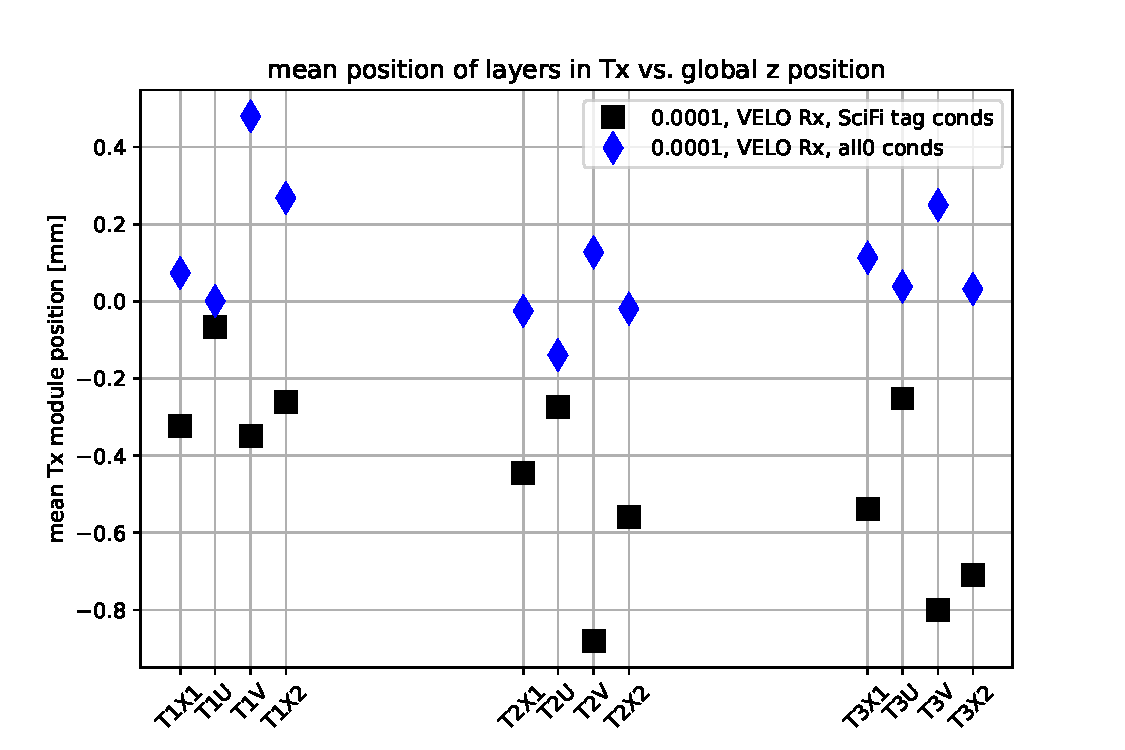
\includegraphics[width=\textwidth]{plots/03-19/all_runs_iD_glob_z_vs_local_Tx.pdf}
      \end{figure}
    \end{column}
    \begin{column}[c]{0.5\textwidth}
      \begin{itemize}
        \item $\bullet$\, SciFi halfmodules: TxRxRz
        \item $\bullet$\, Full VELO Rx
        \item $\bullet$\, fixing SciFi backlayer
        \item $\bullet$\, Black: SciFi alignment tag starting conditions, blue: nominal starting conditions
        \item $\bullet$\, Global alignment seems to working a bit better with blue configuration (\to layers closer to 0)
        \item \to Zig-zag smaller in T2
      \end{itemize}
    \end{column}
  \end{columns}
\end{frame}

\begin{frame}
  \begin{columns}
    \begin{column}[c]{0.5\textwidth}
      After aligning TxRxRz \to alignment wants the Halfmodules in Ry aligned 
      \begin{figure}
        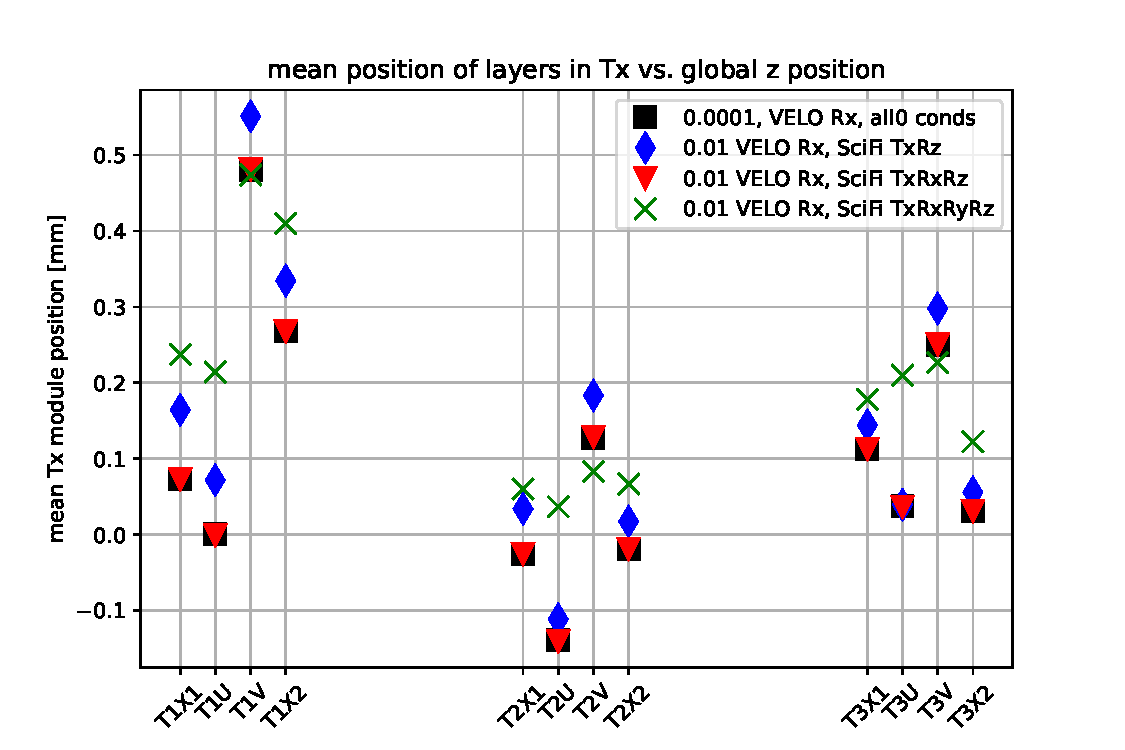
\includegraphics[width=\textwidth]{plots/03-19/all_runs_rx_glob_z_vs_local_Tx.pdf}
      \end{figure}
    \end{column}
    \begin{column}[c]{0.5\textwidth}
      \begin{table}
        \centering
          \begin{tabular}{c c}
          \toprule
            VELO Rx & residual misalignment global VELO \\
          \midrule
            0.0001 & -493.2 \si{\micro\radian} \\
            0.0002 & -505.4 \si{\micro\radian} \\
            0.001  & -506.1 \si{\micro\radian} \\
            0.01   & -389 \si{\micro\radian} \\
          \bottomrule
        \end{tabular}
      \end{table}
      \begin{itemize}
        \item $\bullet$\ Adding Ry alignment improves zig-zag in T2, slightly worse in T1
        \item $\bullet$\ Tx movement somewhat absorbed in Rz
        \item $\bullet$\ VELO Rx does not seem to make a big difference regarding zig-zag pattern
      \end{itemize}
    \end{column}
  \end{columns}
\end{frame}

\begin{frame}
  \begin{columns}
    \begin{column}[c]{0.5\textwidth}
      \begin{figure}
        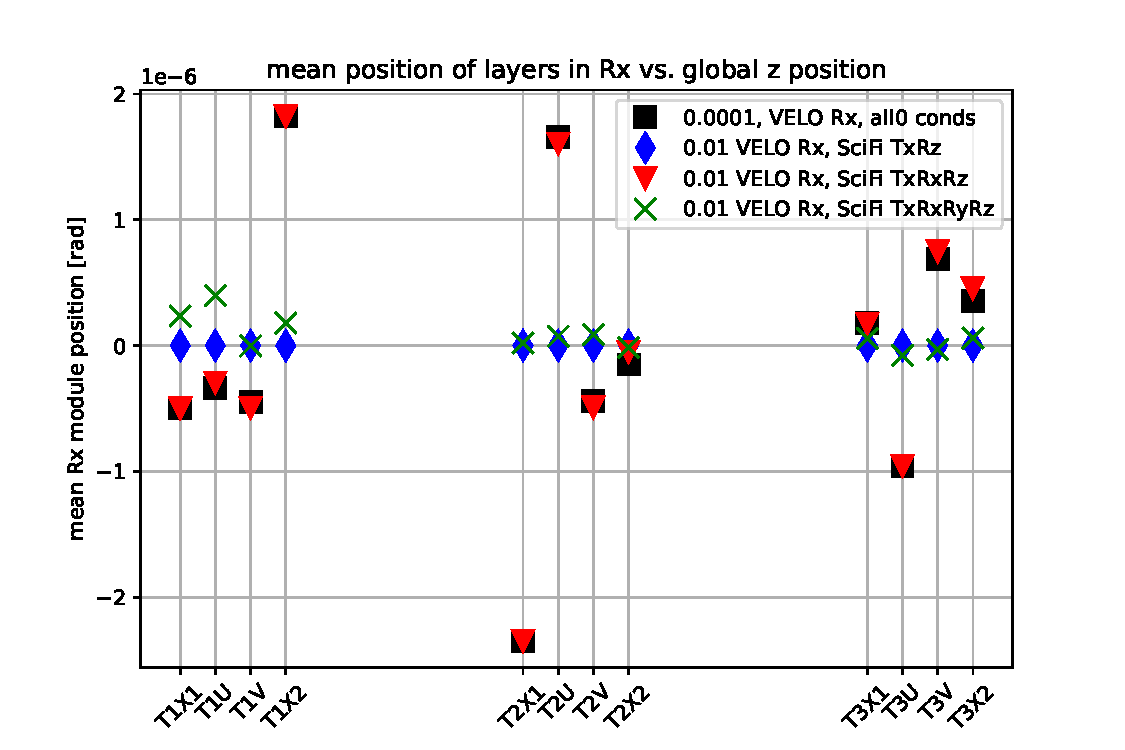
\includegraphics[width=0.9\textwidth]{plots/03-19/all_runs_rx_glob_z_vs_local_Rx.pdf}
      \end{figure}
    \end{column}
    \begin{column}[c]{0.5\textwidth}
      \begin{figure}
        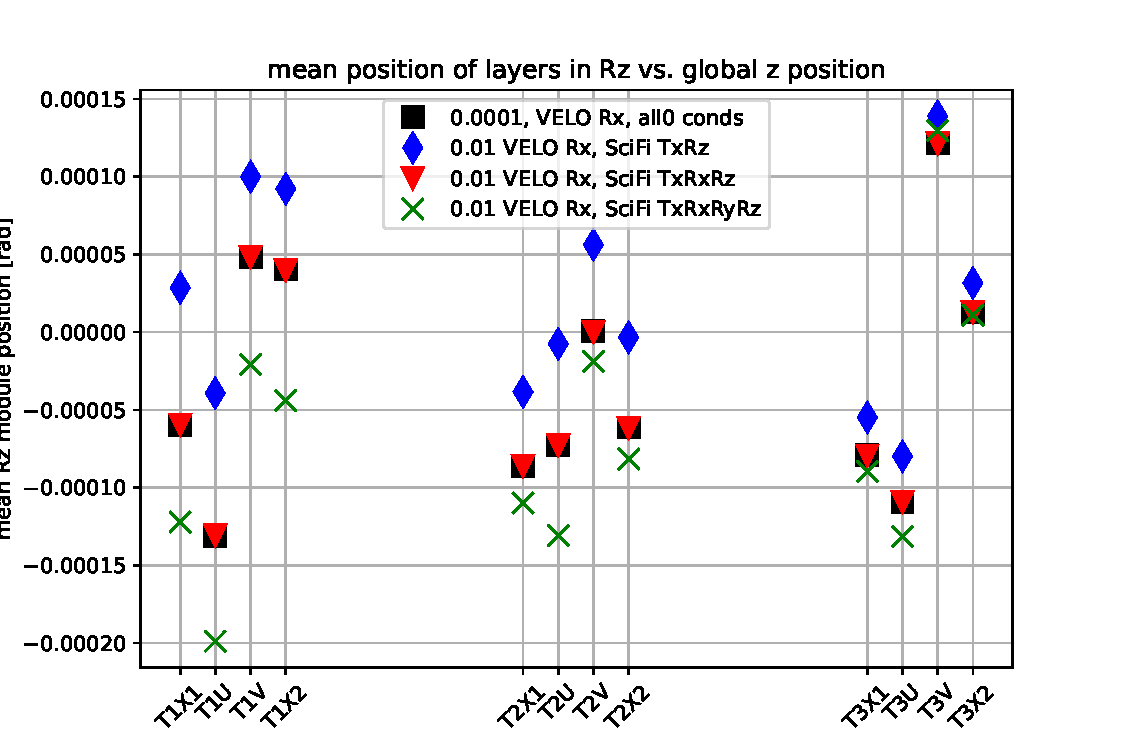
\includegraphics[width=0.9\textwidth]{plots/03-19/all_runs_rx_glob_z_vs_local_Rz.pdf}
      \end{figure}
    \end{column}
  \end{columns}
\end{frame}

\begin{frame}
  \begin{itemize}
    \item $\bullet$\ For global alignment, starting from all 0 positions works better
    \item $\bullet$\ Adding Ry reduces T2 zig-zag pattern. 
    \item $\bullet$\ VELO Rx has a small impact but not the reason for zig-zag pattern
    \item $\bullet$\ We will check this configuration next on 2024 MC
  \end{itemize}
\end{frame}

\begin{frame}
  \begin{figure}
    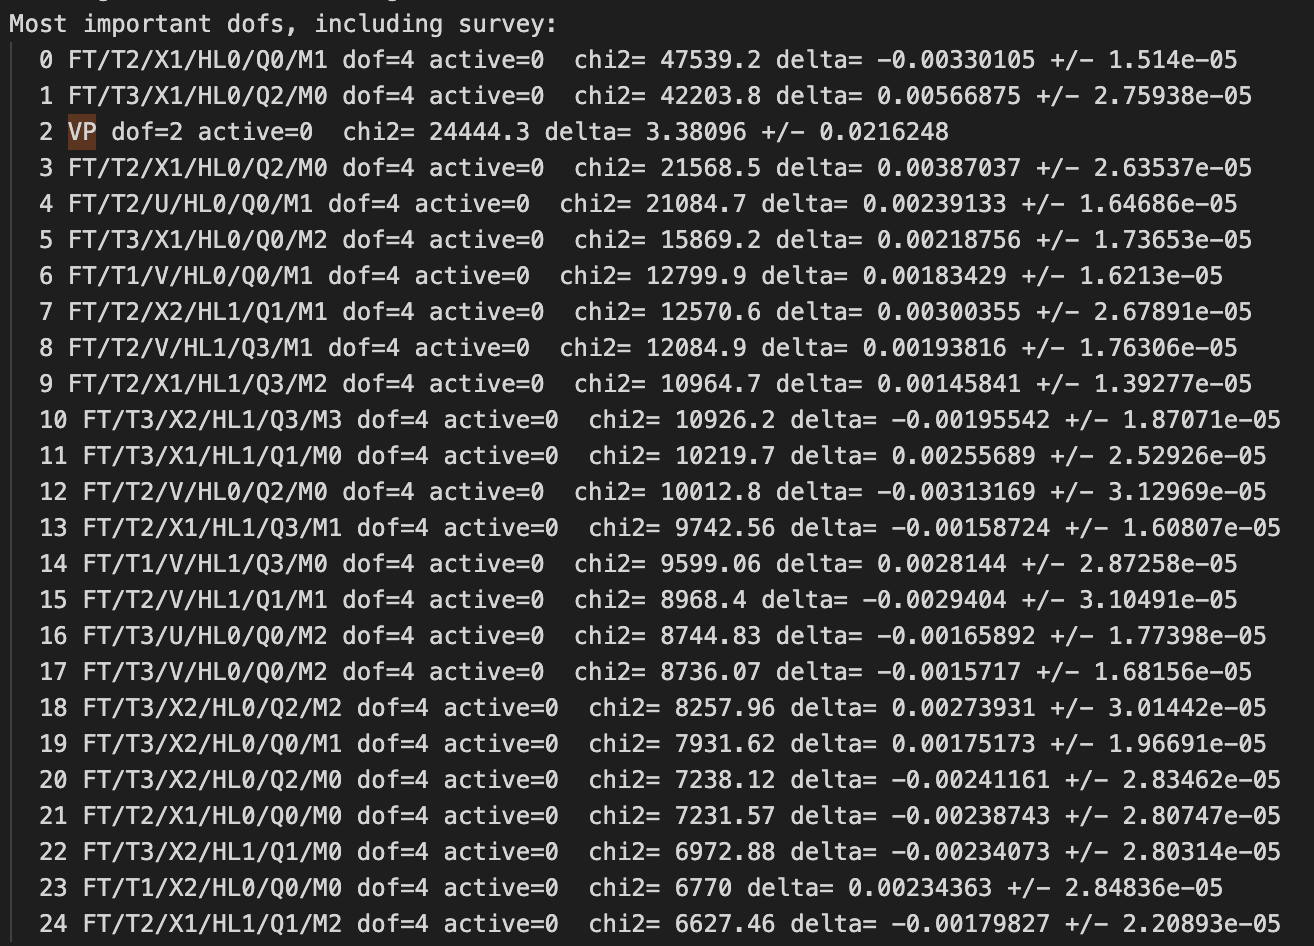
\includegraphics[width=0.7\textwidth]{plots/03-19/dof4.png}
  \end{figure}
\end{frame}

\end{document}
